\documentclass[12pt]{article}

\usepackage{fullpage}
\usepackage[utf8]{inputenc}
\usepackage[T1]{fontenc}
\usepackage{indentfirst}
\usepackage{graphicx}
\usepackage{booktabs}
\graphicspath{ {images/} }
\usepackage[portuguese]{babel}
\usepackage{amsmath}
\usepackage{mathtools}
\usepackage{interval}

\begin{document}
\begin{titlepage}
    
\includegraphics[width=0.3\textwidth]{fctUnlLogo.jpg}
    \begin{center}
        \vspace{0.5cm}

        \begin{Large}
        	{\textbf{State Machine Replication with Multi-Paxos}}\\
        \end{Large}
               
        \vspace{0.3cm}

		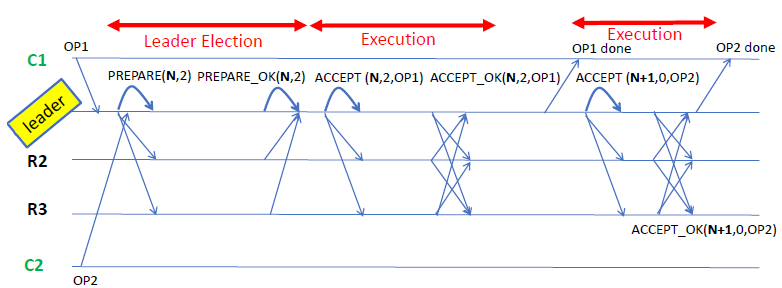
\includegraphics[width=0.9\textwidth]{multipaxos.png}
		
        \vspace{0.3cm}
        
        Trabalho realizado por:
        
        \vspace{0.5cm}

		\begin{table}[htbp]
		\centering
        	\begin{tabular}{c c}
				\textbf{Luís Duarte Oliveira, nº 41894} & \textbf{Daniel Pimenta, nº 45404}\\
				\texttt{ld.oliveira@campus.fct.unl.pt} & \texttt{d.pimenta@campus.fct.unl.pt}\\
			\end{tabular}
		\end{table}
		
		\begin{table}[htbp]
		\centering
        	\begin{tabular}{c}
				\textbf{Luís Martins, nº 45640}\\
				\texttt{lg.martins@campus.fct.unl.pt}\\
			\end{tabular}
		\end{table}
		
        \vspace{0.5cm}
        
        Para a cadeira de:
        
        Algoritmos e Sistemas Distribuídos (ASD)
        
        \vspace{0.5cm}

		Professor regente: 
		João Leitão
		
		Professor responsável:
		Nuno Preguiça
		
        \vspace{0.5cm}
                
        Departamento de Informática\\
        Faculdade de Ciências e Tecnologia\\
        Universidade Nova de Lisboa\\
        17 de novembro de 2018
    \end{center}
\end{titlepage}

\newpage
\tableofcontents

\newpage
\listoffigures

\newpage
\section{Introdução}


\newpage
\section{Visão global}



\newpage
\section{Visão global detalhada}

Nesta secção, iremos explicar por escrito, em pormenor, os detalhes de cada uma das camadas anteriormente mencionadas.

\subsection{Multi-Paxos}

\newpage
\subsection{State Machine Replication}

\newpage
\subsection{Aplicação cliente}


\newpage
\section{Pseudo-código e arquitetura}

Nesta secção, apresenta-se o pseudo-código e uma discussão sobre as propriedades de cada camada do sistema.

\subsection{Multi-Paxos}

\subsubsection{Pseudo-Código}


\bigbreak
\textbf{State:}

\bigbreak
\textbf{Upon Init do:}

\subsubsection{Discussão}


\newpage
\subsection{State Machine Replication}

\subsubsection{Pseudo-Código}

\bigbreak
\textbf{State:}


\bigbreak
\textbf{Upon Init do:}

\subsubsection{Discussão}

\newpage
\section{Avaliação dos resultados}

Esta secção aborda as experiências que se realizaram, os resultados e conclusões das mesmas.

\subsection{Experiências}


\subsection{Resultados com observações}


\newpage
\section{Conclusão}


\newpage
\begin{thebibliography}{00}

\end{thebibliography}

\end{document}